\documentclass[a4paper,13pt,oneside]{article}
 \usepackage[latin1]{inputenc}
 \usepackage[T1]{fontenc}
 %\usepackage[utf8]{inputenc}
 \usepackage[english]{babel}
\usepackage{amssymb}
\usepackage{graphicx}
\usepackage{subfigure}
\usepackage{amsmath}
\usepackage{amsthm}
\usepackage{float}
\usepackage{tikz}
\usepackage{ragged2e}
%\usepackage{ipynb-tex}
\usepackage{pythontex}
\usepackage{minted}
\usepackage{hyperref}
\newtheorem*{claim}{Claim}

\theoremstyle{remark}
\newtheorem*{remark}{Remark}
\renewcommand*\abstractname{\flushleft\textbf{Abstract}\hfill}
\hypersetup{
	colorlinks=true,
	linkcolor=black,
	filecolor=blue,      
	urlcolor=blue,
}
\urlstyle{same}
\title{Betting on Catalan numbers}
\author{Dylan Da Silva Moreira, Hukic Ibrahim}

\begin{document}
\maketitle
\tableofcontents
\newpage



\section{Introduction }

		A fair coin is flipped $100$ times yielding a sequence $a = (a_1,\dots, a_{100})$ of Heads or Tails. Player A realizes that if one thinks of Heads as $+1$ and Tails as $-1$, then for each k\ in [1, 100], $\sum_{i=1}^{k} a_i \geq 0$.
		\\Furthermore, $\sum_{i=0}^{100} a_1=0$.
		\\Player B thinks such a sequence is extremely unlikely and offers a bet to A with a $100 : 1$ odds that if they flip the coin again $100$ times yielding a random sequence $x = (x_1,\dots, x_{100})$, then $x$ is not going to satisfy the properties of $a$. Should A accept the bet? What are the true odds for such an event? Is there a good graphical representation for the properties of $a$? What if there are $2n$ coin flips? Biased coin?
		
\bigskip

\begin{flushleft}
The solution to this problem will be structured in four parts. We start with a practical approach and do some programming and computation to get a feeling for the problem, after plotting our results we move over to find theoretical answer to our problem.Next we calculate the asked probability and check if it matches the probability value obtained in our experiment. Finally we will answer the questions regarding the betting game and what happens in the case of a biased coin. 
\end{flushleft}
\pagebreak
\section{Experiment (Programming)}
%\ipynbsource{Proba}[prog]
\subsection{Program}
\begin{minted}{python}
def verify(s):
  if sum(s) == 0: 
     partial = 0
     for i in s:
         partial = partial + i
         if partial < 0:
            return False
     return True
   return False
   
   
def prob(n):
    count = 0
    for _ in range(n):
        seq = [random.choice([-1,1]) for _ in range(l)]   
        if verify(seq):
           count += 1
    return count/n
	
	\end{minted}
The first function  \textbf{verify}  takes in a sequence $s$ and checks if the given  sequence verifies our conditions by outputting a boolean.
The second function \textbf{prob} computes $n$ sequences of length $l$ and counts how many of these sequences verify our conditions by outputting it's probability.\\

\mintinline{python}{	v = [(x,prob(x))  for x in range(1,n+1)]} \\
\begin{flushleft}

We save the result in a list $v$ of tuples up to $n$ times we want to repeat the experiment.
Now one only needs to plot the list using the \mintinline{python}{list_plot(v)} command.
\end{flushleft}
\pagebreak
\subsection{Results}
The $x$-axis represents the $n$ times we repeat the experiment and the $y$-axis the value of the \textbf{prob} function. 
\begin{center}

	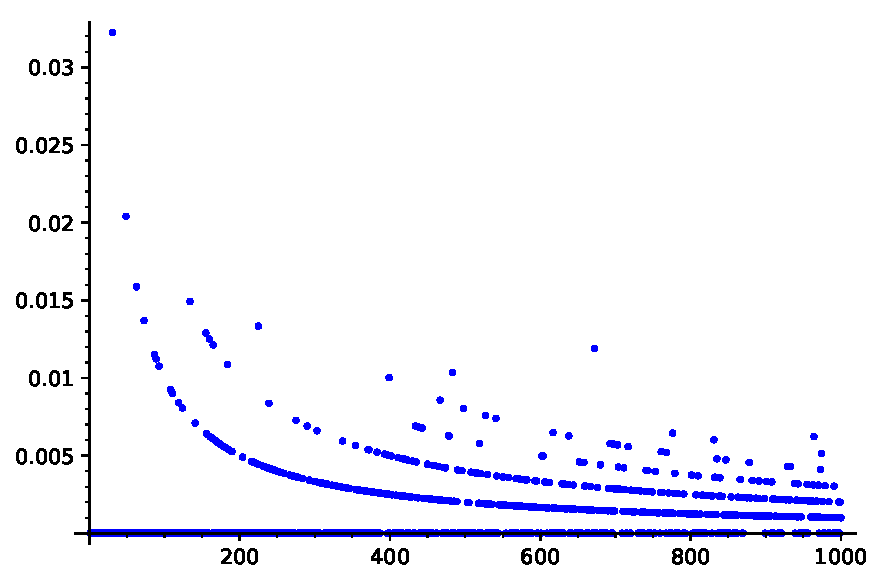
\includegraphics[width=.7\linewidth]{p1.pdf}\\
	For $n=1000$ and $l=100$
\end{center}
\begin{flushleft}
We can see that the probability value does converge as we increase the number of tries.
To have a better overview let us increase $n$ , for computational power reasons we have to decrease the length of the sequence $l$ so the program doesn't take too long. 
\end{flushleft}
\begin{center}
		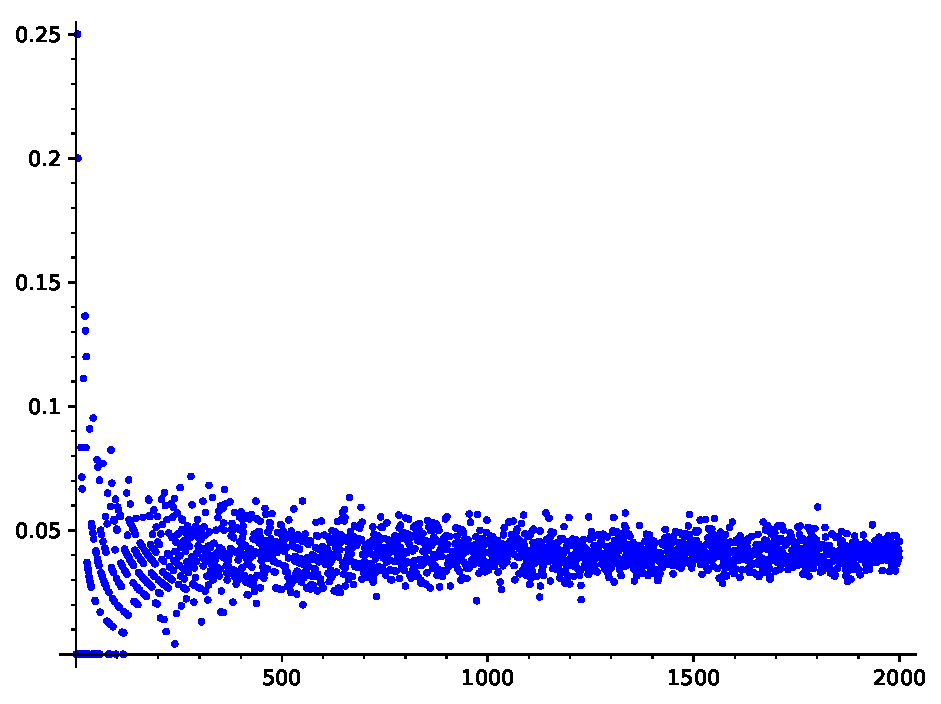
\includegraphics[width=.7\linewidth]{p2.pdf}\\
	For $n=2000$ and $l=10$
\end{center} 
Here we can see that the probability value does converge from both sides to a certain value as we expected.\\
\begin{flushleft}
In both cases one can estimate the value to be around $0.002$ for $l=100$ and $0.05$ for $l=10$.
The next step will be to determine this exact value and if does match our approximation from the experiment. 
\end{flushleft}
  
	
\pagebreak
\section{Theoretical approach}
\subsection{Preparation}

Let us redefine our $+1$,$-1$ random sequence into \textit{rightward} ($-1$) and \textit{upward} ($+1$) steps. The solution to our coin flip problem are all the paths that end on the straight line $f(x) = x$ (sum equals to zero) and don't cross the line at any given moment (sum being always positive).

\bigskip


\begin{center}

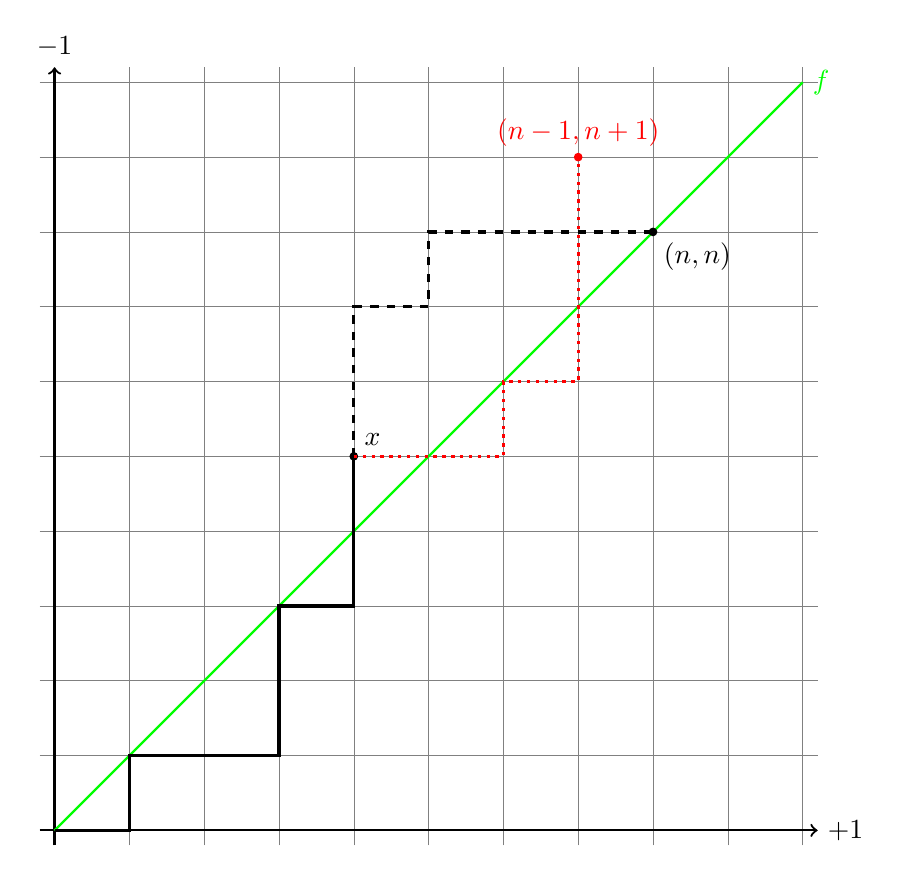
\begin{tikzpicture}[scale= 0.95]
\draw[gray, very thin] (-0.2,-0.2) grid (10.2,10.2);
\draw[->,thick] (-0.2,0) -- (10.2,0) node[right]{$+1$} ; 
\draw[->,thick] (0,-0.2) -- (0,10.2) node[above] {$-1$} ;
\draw[green ,thick] (0,0) -- (10,10) node[right] {$f$};
\draw [very thick](0,0) -- (1,0) -- (1,1) -- (3,1) -- (3,3) -- (4,3) --(4,5) node[above right] {$x$};
\draw [fill] (4,5) circle[radius=0.05];
\draw [dashed, very thick] (4,5) -- (4,7)--(5,7)--(5,8)--(8,8) node[below right]{$(n,n)$};
\draw [fill] (8,8) circle[radius=0.05];
\draw[dotted,very thick,red]   (4,5)--(6,5)--(6,6)--(7,6)--(7,9) node[above] {$(n-1,n+1)$};
\draw[fill,red] (7,9) circle[radius=0.05];
\end{tikzpicture}

\end{center}


\begin{claim} \label{claim}
The number of paths satisfying the above conditions is given by:
\[
\boxed{\binom{2n}{n} - \binom{2n}{n+1}  \quad ,n\in \mathbb{N}}
\]	
\end{claim}
\bigskip
\begin{remark}
A point on the line $f$ is denoted by $(n,n)$ where $n =\frac{l}{2}$ with $l$ being the length of the sequence.
\end{remark}
\bigskip
\begin{proof}
To end up at the point $(n,n)$ one has to choose $n$ \textit{upward} (or equivalently \textit{rightward}) steps out of $2n$ total steps. So the number of paths satisfying this condition is equal to : 
\[\binom{2n}{n}\] 
Considering this number still contains paths which will end on the line but cross it at a given moment we need to exclude them.
To find out the number of "bad paths" we will flip the portion of a path \underline{after}  it has crossed the line for the first time. By "flipping" one means interchanging all  \textit{upwards} and \textit{rightward} steps.
The section of a bad path which hasn't been flipped contains one more \textit{upwards} step than \textit{rightward} steps, hence the remaining path contains one more \textit{rightward} step than \textit{upward} step because it end on the line $f$. Since there are $2n$ steps and the flipping process doesn't change the total amount of steps , every flipped bad path will ends at the point $(n-1,n+1)$.
Thus the number of bad paths is given by the possible permutations of $n+1$ \textit{upward} steps (or equivalently, $n-1$ \text{rightward} steps)  for a total of $2n$ steps : 
\[
\binom{n+1+n-1}{n+1} =\binom{2n}{n+1}= \binom{2n}{n-1}
\]

By subtracting  one finally obtains :
\[
\binom{2n}{n} - \binom{2n}{n+1}
\]


\end{proof}
\bigskip

Let us develop this expression furthermore :
\begin{align*}
\binom{2n}{n} - \binom{2n}{n+1} &= \frac{(2n)!}{n! \, (2n-n)!} - \frac{(2n)!}{(n+1)! \, (2n-n-1)!}\\
&= \frac{(2n)!}{n! \, (2n-n)(2n-n-1)!} - \frac{(2n)!}{(n+1)\,n! \, (2n-n-1)!}\\
&= \frac{(2n)! \, (n+1-2n+n)}{n!\,(2n-n-1)!\,(2n-n)(n+1)}\\
&=\frac{(2n)!}{n!\,(2n-n-1)!\,(2n-n)(n+1)}\\
&= \frac{(2n)!}{n!\,(2n-n)!\,(n+1)} = \frac{(2n)!}{(n+1)! \,n!}\\
&= \frac{1}{1+n} \binom{2n}{n}
\end{align*}

\begin{flushleft}
One realizes that this is the formula for the \textbf{Catalan numbers}, which is a sequence of natural numbers given by :
\[ 
\boxed{C_n = \frac{1}{1+n} \binom{2n}{n}= \frac{(2n)!}{(n+1)! \,n!}=\prod_{k=2}^{n} \frac{n+k}{k} \qquad \text{for} \:n \geq 0.}
\]
\end{flushleft}
\pagebreak
\subsection{The expected value}
Now one can easily determine the probability of such a sequence to occur. Let's call this probability $P_{100}$ for the sequence of length $100$ and $P_{10}$ for the sequence of length $10$ :

\begin{align}
P_{100} &= \frac{C_{50}}{2^{100}} = 0.0015605732821015443431 \simeq 0.00156 \\
P_{10} &= \frac{C_5}{2^{10}} = 0.041015625 \simeq 0.041 
\end{align}

\begin{remark}
Notice that the Catalan number $C_{50}$ it the number of possibilities satisfying our condtions for a length $l = 100$ since we defined $n=\frac{l}{2}$. Analogously for $C_5$.
\end{remark}
\bigskip
Let's see if these values correspond to our estimations:
\begin{center}
		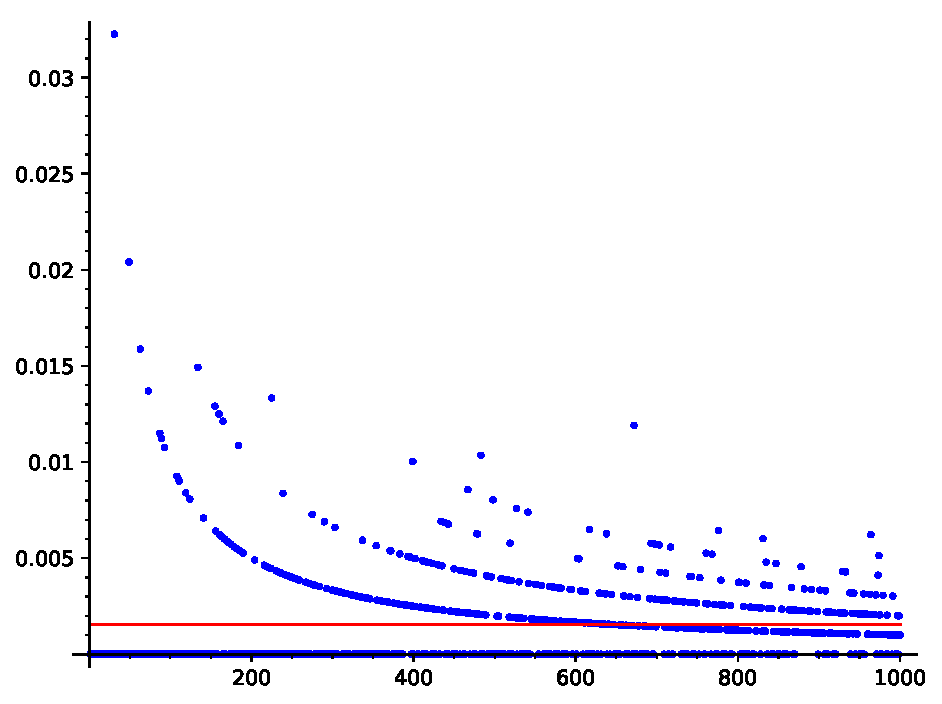
\includegraphics[width=.7\linewidth]{p12.pdf}\\
	For $n=1000$ and $l=100$
		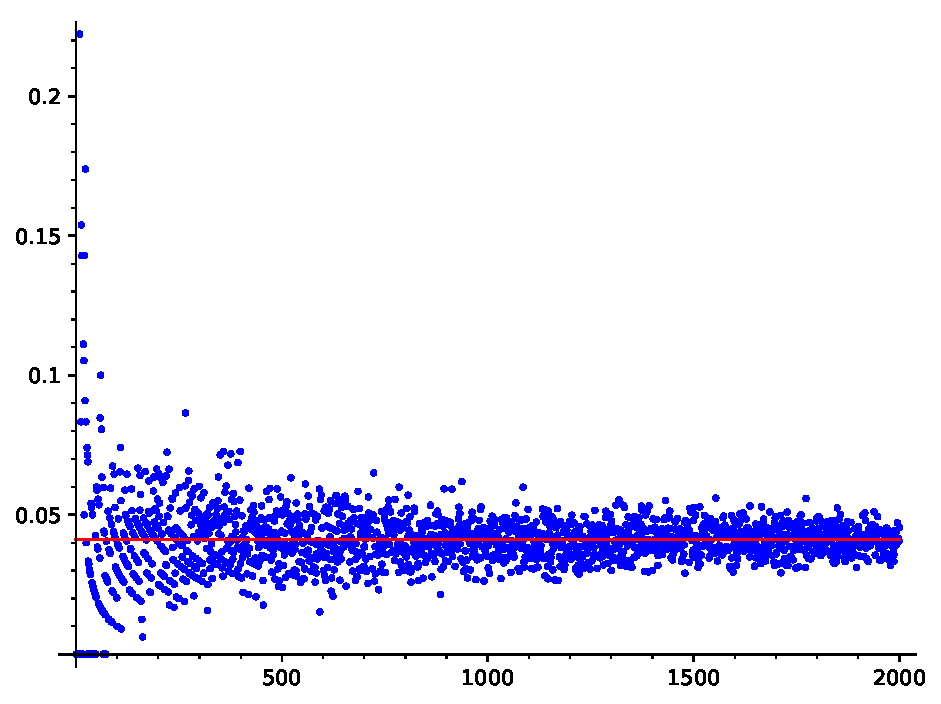
\includegraphics[width=.7\linewidth]{p22.pdf}\\
	For $n=2000$ and $l=10$
	
\end{center}
Indeed, in both cases they converge to our calculated value (red line).
 \pagebreak
\section{Outcome}
\subsection{What should player $A$ do ?}
In this section we will discuss if player $A$ should accept the bet, if not under which conditions should  he play such that the bet would be in his favour.\\
To answer this question it suffices to calculate the \textit{expected value} $E[X]$, where $X$ is a random variable and represents the outcome of  either "winning 100eur" or "loosing 1eur". Since one has only two possible outcomes this is fairly easy:
\[
E[X]= 100 \,P_{100} -(1-P_{100}) = -0.84238209850774402135
\] 
Thus player $A$ shouldn't accept the bet under a $100:1$ ratio.
\bigskip
The answer to the second part it suffices to solve the following  inequality where $m$ represents the winning amount of money:
\[
m \,P_{100} -(1-P_{100}) > 0 \iff m > \frac{(1-P_{100})}{P_{100}} = 639.79015799459995134
\]
Let us suppose cents coins are not accepted in this bet, then
the bet is favourable for player $A$ if he accepts to play under a ratio of $640:1$
 
\subsection{Biased coin and Markov Model}
To answer the question in the case of a biased coin we will use the Markov Model to visualize our results.
In order to do that we will take advantage of the implemented function \textit{hmm.DiscreteHiddenMarkovModel} in Sage:\\
\begin{flushleft}

a$=$hmm.DiscreteHiddenMarkovModel([[1/3,2/3],[1/2,1/2]], [[1,0],[0,1]],  [0.5,0.5],[-1, 1])\\
\begin{minted}{ruby}
	[1/3,2/3]
	[1/2,1/2]
	designs the transition matrix
	[1,0]
	[0,1]
	designs the emission matrix
	[0.5,0.5] is the initial probabilty condition and [-1,1] are the respective outcomes

\end{minted}
for detailed description visit: \url{http://doc.sagemath.org/html/en/reference/stats/sage/stats/hmm/hmm.html}\\
Notice that in order to make it a normal Markov model we use the identity matrix as the emission matrix.

\end{flushleft}
Now we can use \mint{Python}{a.sample(l)} to sample a sequence of length $l$ that obeys our biased coin,to write the following program: \\ 


\begin{minted}{python}
def prob_markov(n):
	count = 0
	for _ in range(n):
	  seq = a.sample(l)
	  if verify(seq):
	    count += 1
	
	return count/n

\end{minted}
By saving this in a list as we did in section 2 and plotting it we get:
\begin{minted}{python}
w = [(x,prob_markov(x))  for x in range(1,n+1)]
list_plot(w)
\end{minted}
\begin{center}
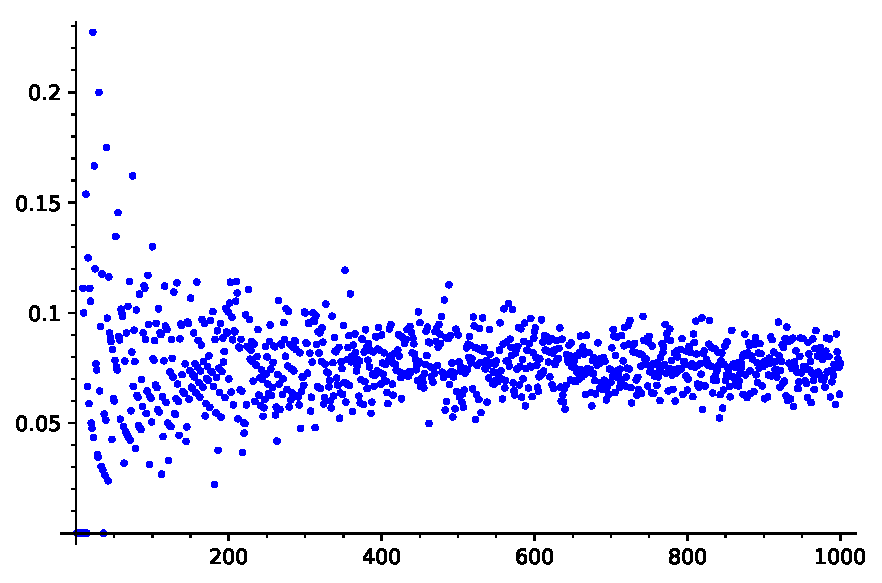
\includegraphics[width=.7\linewidth]{m.pdf}\\
For $n=2000$ and $l=10$
\end{center}

One observes that the probability value of \textbf{prob\_markov} function converges to a different value in the case of a biased coin.\\
The reader is welcome to play around with the program sheet and see how the graph changes accordingly to changes in the transitions matrix .

\section*{Reminder}

We have created a interactive Jupyter sheet which contains all the programs and plots used , you are welcome to play around with. The sheet and the whole presentation has been put in Github repository which can be accessed \href{https://github.com/DaSilvaMoreira/Betting_Game}{HERE}. In order to use this sheet make sure you are using the SageMath Kernel in Jupyter Notebook. It is also worth noticing that to compile the .tex file you must use the \mint{ruby}{pdflatex -synctex=1 -interaction=nonstopmode --shell-escape \%.tex} command in your texeditor.


\end{document}
